\documentclass[main]{subfiles}


\title[AutoML: Introduction]{AutoML Motivation}
\subtitle{How to Use AutoML?}
\author[Marius Lindauer]{Marius Lindauer}
\date{}

\titlebackground*{images/AutoML_AutoDL}

%\institute{}
%\date{}

\begin{document}
	
	\maketitle
	

%----------------------------------------------------------------------
%----------------------------------------------------------------------
\begin{frame}[c]{Interfaces to AutoML: Data-Model}

\begin{columns}

\column{0.5\textwidth}

\centering
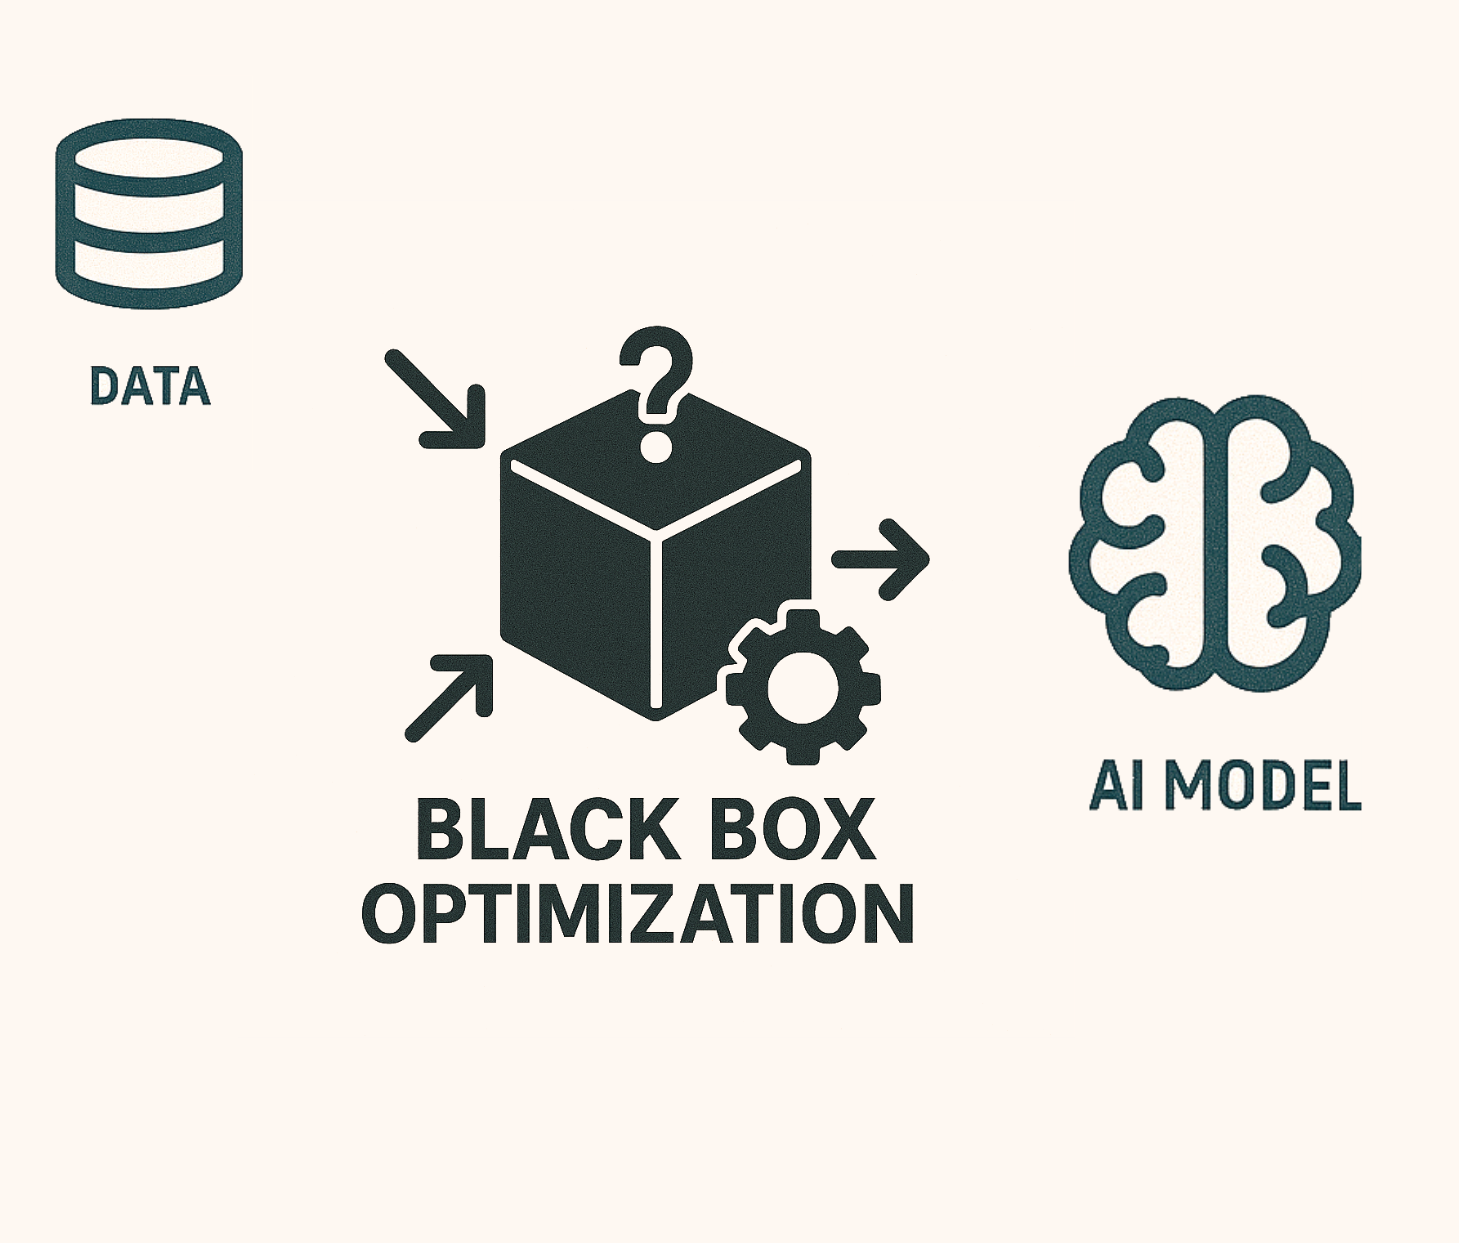
\includegraphics[width=0.8\textwidth]{images/interface_data_model.png}


\column{0.5\textwidth}

\begin{itemize}
    \item Holy grail because it is the easiest interface
    \begin{itemize}
        \item However, in practice, we often need more than that (incl. metric to be optimized for)!
    \end{itemize}
    \item Input: Dataset
    \begin{itemize}
        \item explicitly or implicitly also defines tasks (e.g., labels, supervised vs self-supervised, data modality, etc pp)
    \end{itemize}
    \item Output: Predictive Model 
    \begin{itemize}
        \item Comes often along with further statistics, e.g., expected generalization performance
    \end{itemize}
\end{itemize}
    
\end{columns}

\end{frame}
%-----------------------------------------------------------------------
%----------------------------------------------------------------------
\begin{frame}[c]{Interfaces to AutoML: Data-Constraint-Model}

\begin{columns}

\column{0.5\textwidth}

\centering
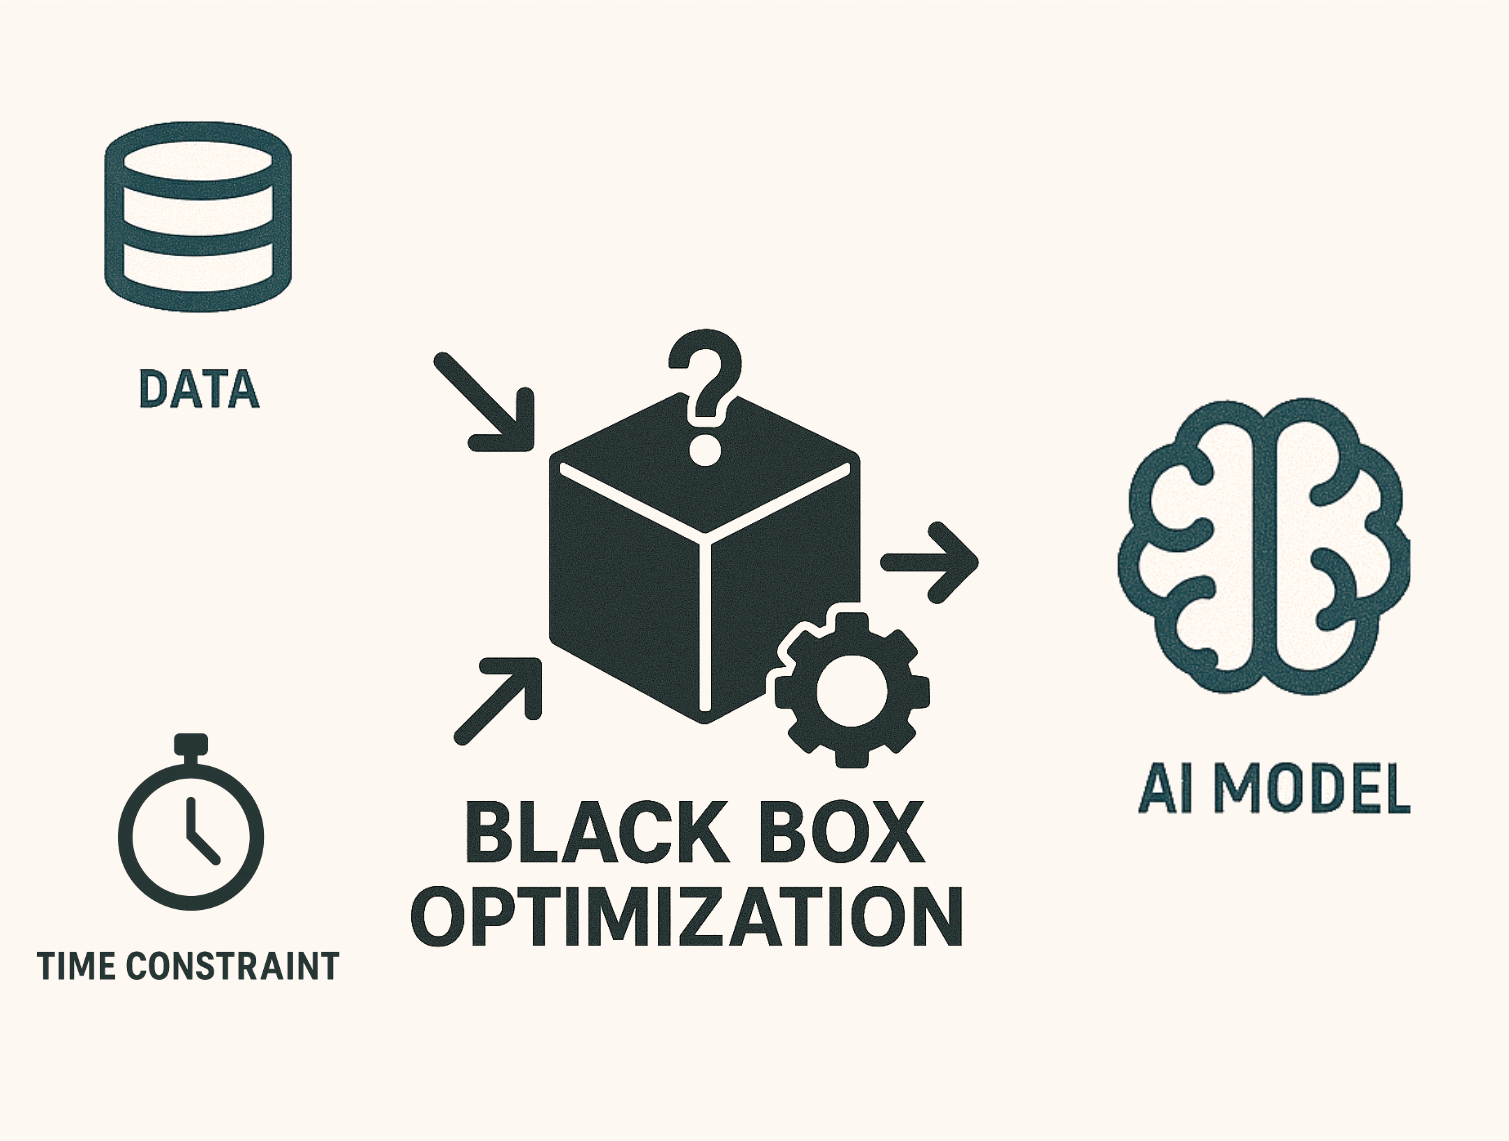
\includegraphics[width=0.8\textwidth]{images/interface_data_constraint_model.png}


\column{0.5\textwidth}

\begin{itemize}
    \item In addition to a dataset being provided and the model as an output, any kinds of constraints, for example:
    \begin{itemize}
        \item Time or compute constraint on the AutoML process
        \item Efficiency constraint on the model being returned
    \end{itemize}
\end{itemize}
    
\end{columns}

\end{frame}
%-----------------------------------------------------------------------
%----------------------------------------------------------------------
\begin{frame}[c]{Interfaces to AutoML: Data-Space-Model}

\begin{columns}

\column{0.5\textwidth}

\centering
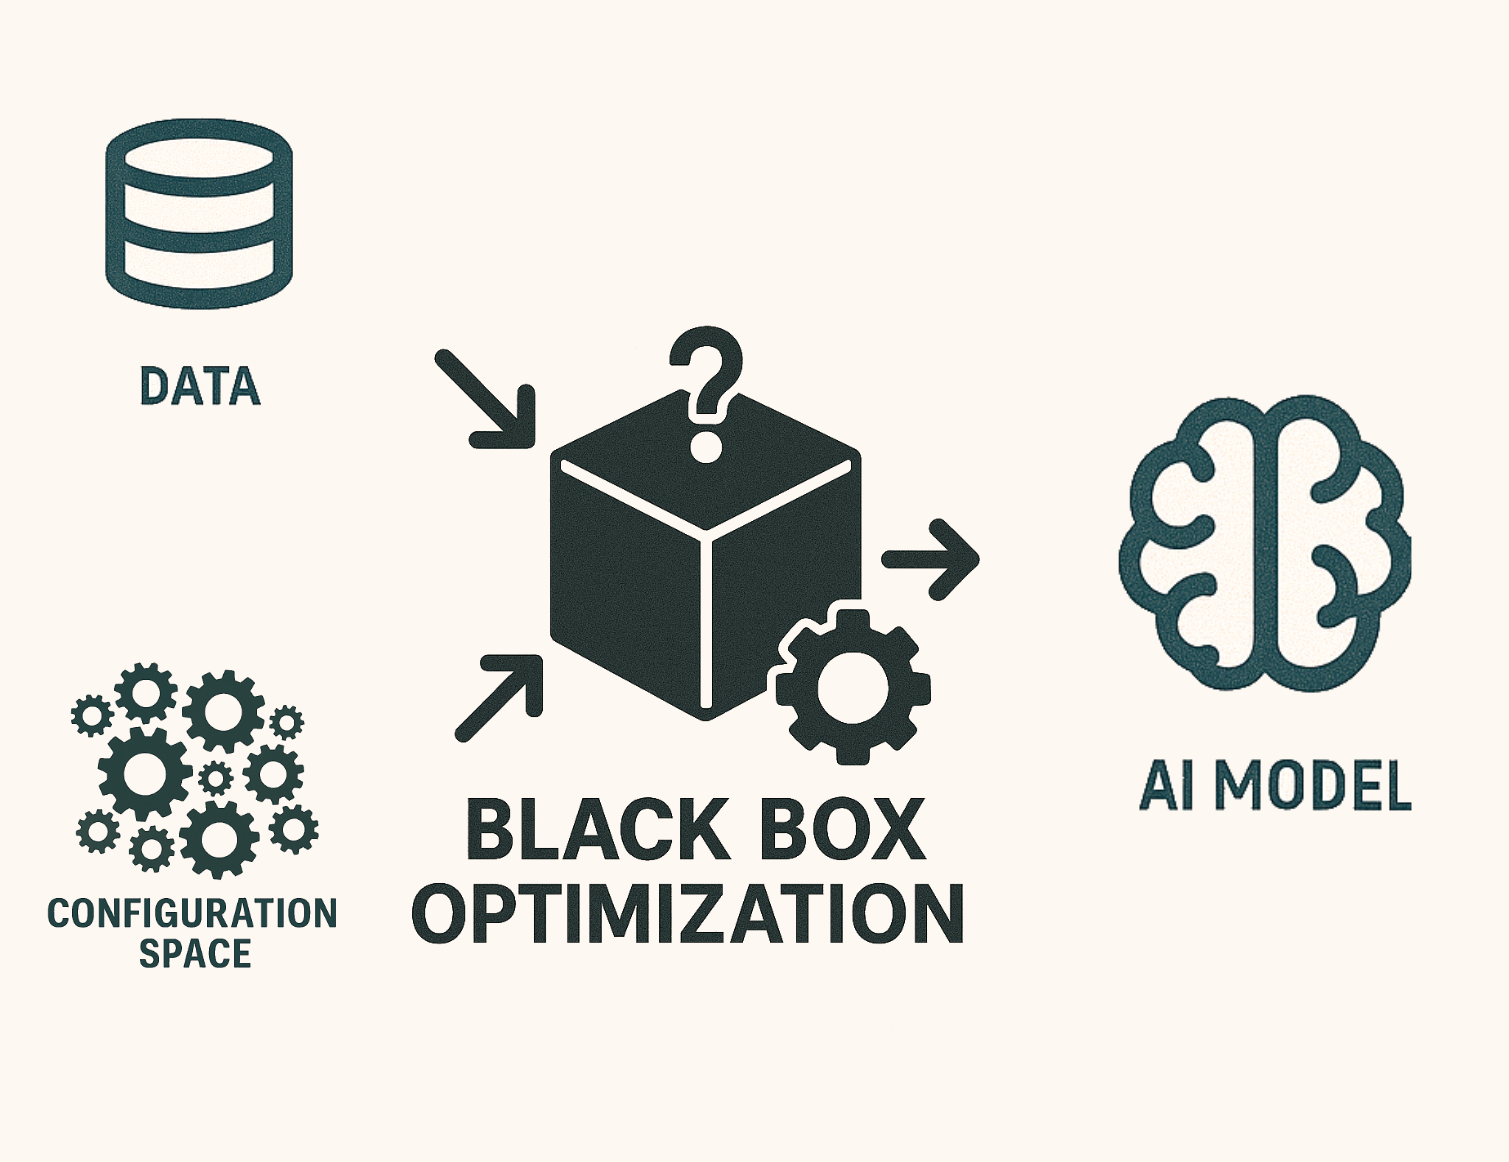
\includegraphics[width=0.8\textwidth]{images/interface_data_space_model.png}


\column{0.5\textwidth}

\begin{itemize}
    \item In contrast to the previous interface, developers might want to define the configuration space themselves (e.g., to constraint certain aspects such as time, efficiency)
    \item Full control of what is actually considered
    \item[$\leadsto$] Can provide efficiency gains by leveraging human expertise
    \item[$\leadsto$] Requires more human expertise
\end{itemize}
    
\end{columns}

\end{frame}
%-----------------------------------------------------------------------
%----------------------------------------------------------------------
\begin{frame}[c]{Interfaces to AutoML: Data-Space-Configuration}

\begin{columns}

\column{0.5\textwidth}

\centering
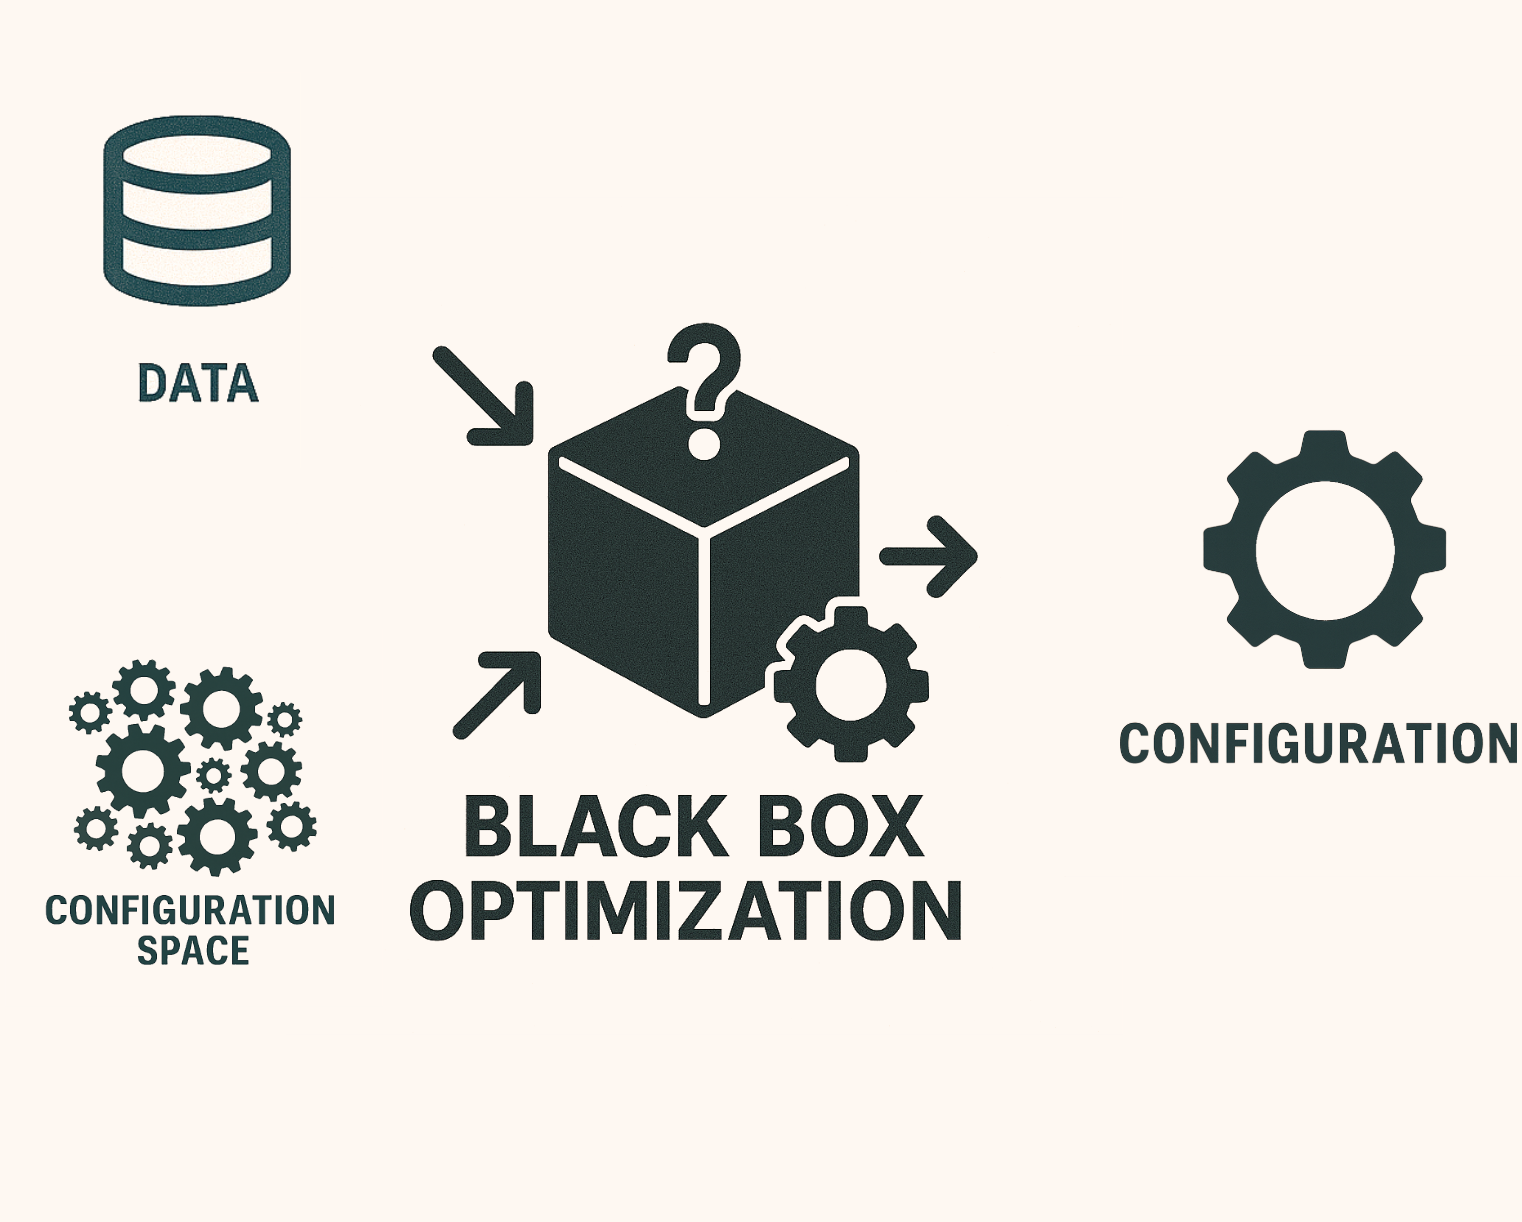
\includegraphics[width=0.8\textwidth]{images/interface_data_space_config.png}


\column{0.5\textwidth}

\begin{itemize}
    \item Rather than returning a model, sometimes we are rather interested in the optimized configuration of the inducer or the entire pipeline
    \item Allows reuse of a configuration if retraining is required or if training on a (very) similar dataset is planned
    \item Can provide more insights than only having the model (e.g., which hyperparameter was important to obtain a performant model)
    \begin{itemize}
        \item Some AutoML tools also return model and configuration
    \end{itemize}
\end{itemize}
    
\end{columns}

\end{frame}
%-----------------------------------------------------------------------
%----------------------------------------------------------------------
\begin{frame}[c]{Interfaces to AutoML: Data-Docu-Code}

\begin{columns}

\column{0.5\textwidth}

\centering
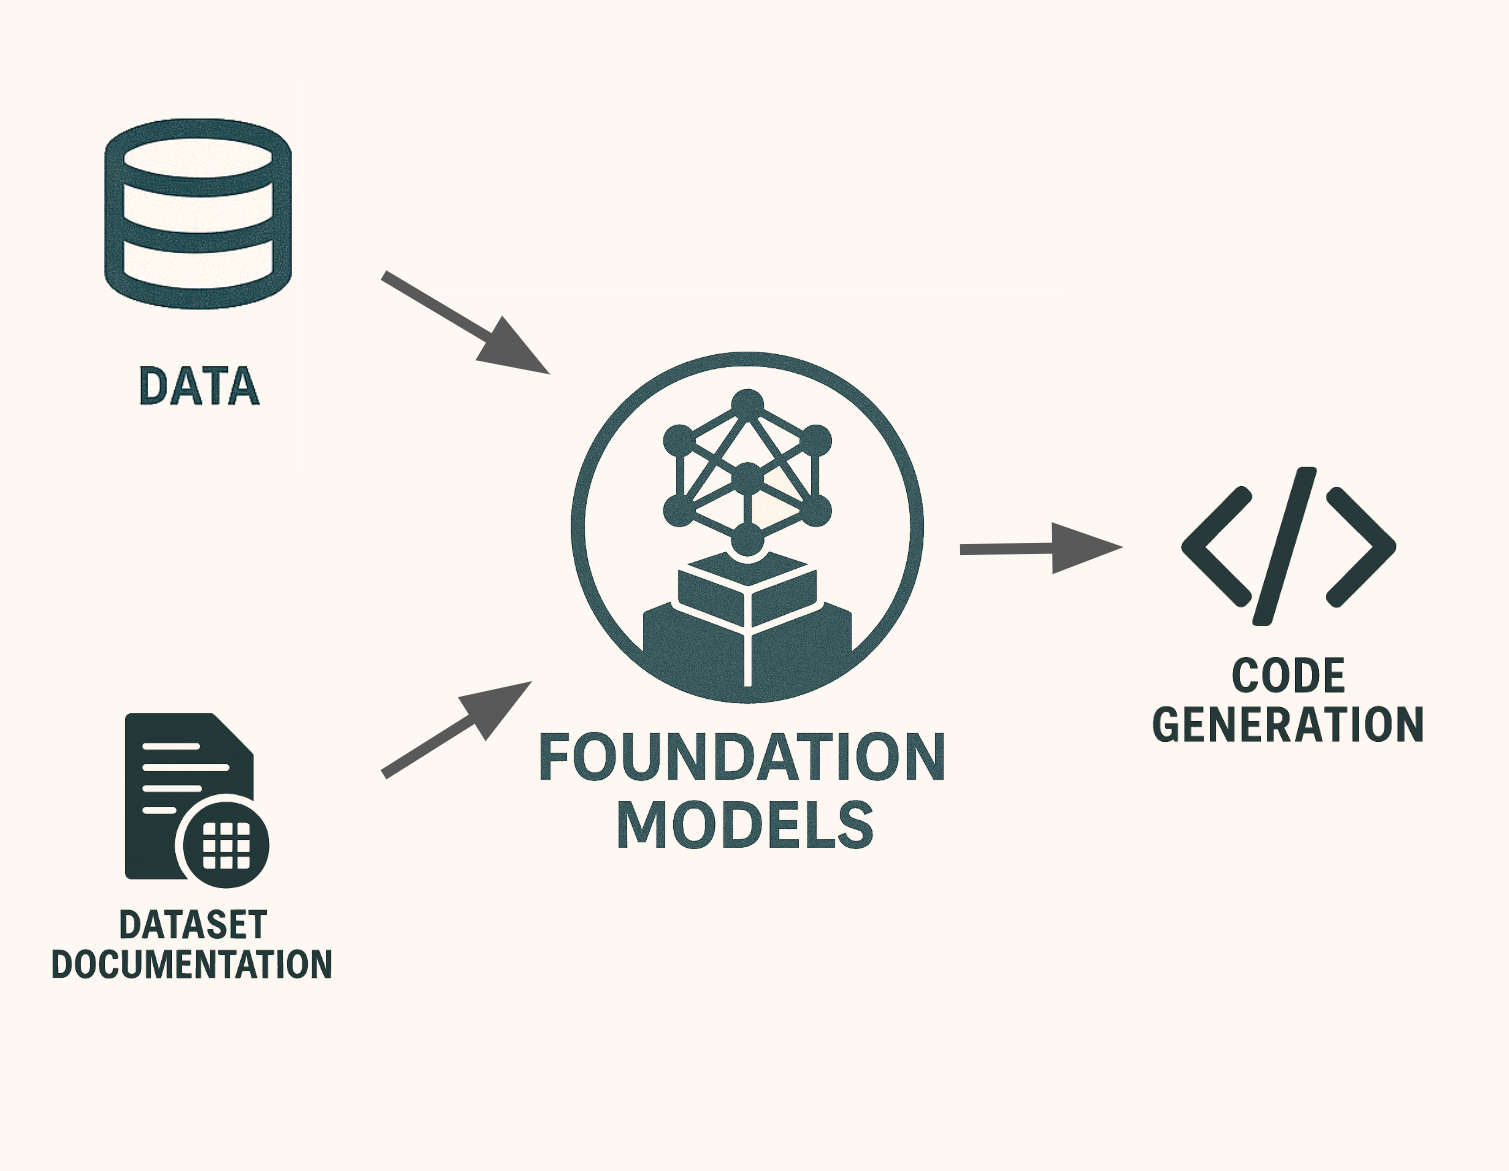
\includegraphics[width=0.8\textwidth]{images/interface_data_docu_code.png}


\column{0.5\textwidth}

\begin{itemize}
    \item Foundation models (e.g., agentic systems) can be used to generate code which allows for 
    \begin{itemize}
        \item more flexibility (compared to a configuration space)
        \item reusing the code 
        \item better understanding (?)
    \end{itemize}
    \item \alert{Extreme case} of this: Only the task description is given, and an agentic system obtains the necessary training data from the web on its own
\end{itemize}
    
\end{columns}

\end{frame}
%-----------------------------------------------------------------------
%----------------------------------------------------------------------
\begin{frame}{Summary} 

Most important insights from this video:

\begin{enumerate}
    \item Although all of these interfaces solve the same AutoML problem, they start with different inputs and return different outputs
    \begin{itemize}
        \item Outputs of AutoML can entail a lot of things in general, incl.\ an ensemble of models, clean data, a prompt, a fine-tuned model, a compressed model, an architecture or code
    \end{itemize}
    \item It depends on the use case and context which interface makes more sense
    \begin{itemize}
        \item For example, domain experts may prefer a very basic interface with a dataset as input and a model as an output
        \item However, ML experts require more control by defining a configuration space and are looking to better understand the final configuration being returned
    \end{itemize}
\end{enumerate}


\end{frame}

\end{document}

